\section{Situation}
Nous devons étre capable d'estimer la valeur $\alpha$ à partir de $y$. Nous disposons des valeurs suivantes (voir la figure~\ref{balis_sit}, page~\pageref{balis_sit}) :
\begin{description}
	\item[$y$] C'est la distance au centre de la cible du point d'impact. Il est choisi aléatoirement en fonction du niveau de difficulté.
	\item[$\alpha$] L'angle de tir. C'est la valeur sur laquelle peut jouer notre robot, le canon étant monté sur un moteur.
	\item[$s$] La taille de la cible. C'est une constante, la taille de la cible ne devant pas varier.
	\item[$c_x$] C'est la distance de la cible au robot. Elle est mesurée en début de partie par un capteur de distance.
	\item[$d_x$] C'est le décalage sur l'axe x entre le capteur de distance et le canon. C'est une constante déterminée au montage du robot.
	\item[$x$] C'est la distance du canon à la cible sur l'axe x. Elle définit comme $x=c_x+d_x$.
	\item[$d_y$] C'est le décalage sur l'axe y entre le capteur de distance et le canon. C'est une constante déterminée au montage du robot.
	\item[$\overrightarrow{v}$] C'est la vitesse de la bille à la sortie du canon. C'est une constante déterminée par des tests.
\end{description}
Toutes les valeurs de distances sont exprimées en $mm$.

Comme vous pouvez le constater, lors d'un tir toutes les valeurs sont connues à l'exception de $\alpha$, $y$ ayant déjà été déterminé pour le tir. Il faut donc trouver la fonction donnant l'angle $\alpha$ pour une position sur la cible $y$ donnée. Afin de simplifier les calculs, on considère que le capteur de distance du robot est en face du centre de la cible et que le robot est bien placé en face de la cible. Les calculs se feront effectivement en deux dimensions.

\begin{figure}
	\begin{center}
		\begin{tikzpicture}[scale=1.5]
			% La cible
			\draw (5,1) -- (5,-1);
			\draw (4.9,1) -- (5.1,1);
			\draw (4.9,-1) -- (5.1,-1);
			\draw (4.9,0) -- (5.1,0);

			% Le canon
			\draw (-1,0.5) -- (-1,-0.5);
			\draw (1,0.5) -- (1,-0.5);
			\draw (1,0.5) -- (-1,0.5);
			\draw (1,-0.5) -- (-1,-0.5);
			\draw (-0.2,0.5) -- (0.3,1);
			\draw (0,0.5) -- (0.4,0.9);
			\draw (0.3,1) -- (0.4,0.9);

			% Les mesures
			\draw[->,thick,blue,dotted] (0.35,0.95) .. controls (2,2.5) and (3,2.5) .. (5,0.6);
			\draw[thick,red,->] (0.35,0.95) -- node[above,red] {$\overrightarrow{v}$} (1,1.6);
			\draw[<->,thick,green] (1.1,0) -- node[black,below] {$c_x$} (4.8,0);
			\draw[<->,green] (0.9,0) -- node[black,below] {$d_x$} (0.1,0);
			\draw[<->,green] (0,0.1) -- node[black,left] {$d_y$} (0,0.4);
			\draw[<->] (5.2,1) -- node[black,right] {$s$} (5.2,-1);
			\draw[<->,blue] (5.6,0) -- node[black,right] {$y$} (5.6,0.6);

			% L'angle
			\filldraw[fill=green!20!white, draw=green!50!black]
			(0,0.5) -- (0.4,0.5) arc (0:60:3mm) node[black,right]{$\alpha$} -- cycle;
		\end{tikzpicture}
	\end{center}
	\caption{Situation de tir.}
	\label{balis_sit}
\end{figure}

\section{Calculs}
On obtient la fonction de la trajectoire ($g$ étant l'accélération gravitationnelle, une constante liée sur terre ayant pour valeur $g = 10000\ mm.s^{-1}$) :\begin{equation}
	traj(p) = -g*\frac{p^2}{2*\overrightarrow{v}^2*cos(\alpha)^2} + p * tan(\alpha) + d_y
\end{equation}

La figure~\ref{crb_traj} (page~\pageref{crb_traj}) montre la trajectoire obtenue pour des valeurs arbitraires de : \begin{itemize}
	\item $v = 7000\ mm.s^{-1}$
	\item $\alpha = 44$
	\item $d_y = 0$
\end{itemize}

En effet, ces valeurs n'ont pas encore été mesurées au moment de la rédaction de ce compte rendu. Tous les graphiques ultérieurs utiliseront donc des valeurs arbitraires.

\begin{figure}
	\begin{center}
		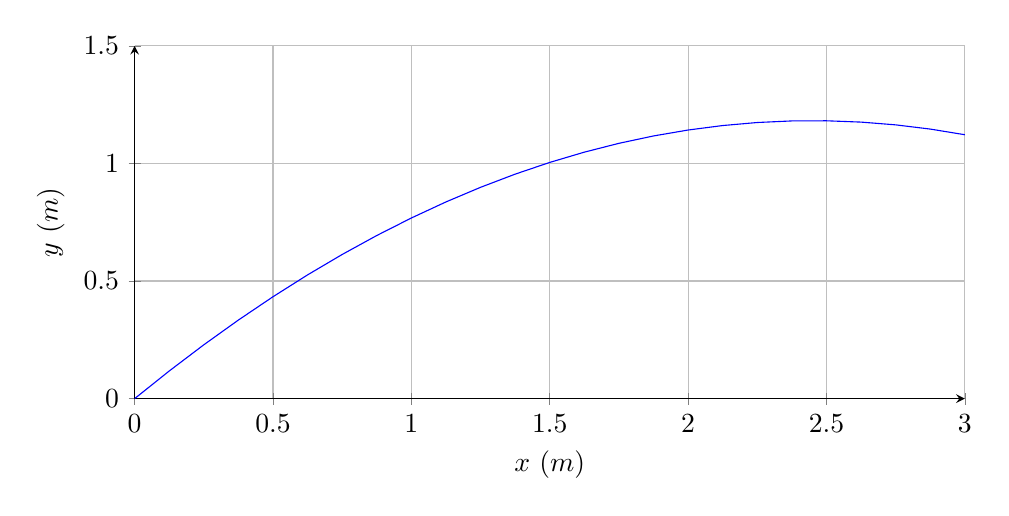
\begin{tikzpicture}
			\begin{axis}[height=0.5\linewidth, width=\linewidth,
					axis x line=bottom, axis y line=left, grid=major,
					xlabel={$x\ (m)$}, ylabel={$y\ (m)$},
				xmin=0, xmax=3, ymin=0, ymax=1.5]
				\addplot+[mark=none,domain=0:3] {-0.197*x*x+x*0.965};
			\end{axis}
		\end{tikzpicture}
	\end{center}
	\caption{Trajectoire du projectile.}
	\label{crb_traj}
\end{figure}

On travaille maintenant la formule de la trajectoire pour lier l'angle de départ à la hauteur sur la cible. La hauteur sur la cible correspond à l'image de la distance canon-cible par la fonction de la trajectoire. On remplace donc cette valeur dans la fonction par la distance mesurée au début de chaque jeu. Dans les exemples suivants, on considérera que cette valeur vaut $x = 2000\ mm$. Puis on passe l'angle en paramètre. On obtient donc une fonction qui nous donne la hauteur sur la cible selon l'angle de tir :\begin{equation}
	h(\alpha) = -g*\frac{x^2}{2*\overrightarrow{v}^2*cos(\alpha)^2} + x*tan(\alpha) +d_y
\end{equation}

On peut donc dessiner une courbe indiquant la hauteur sur la cible en fonction de l'angle de départ; c'est la figure~\ref{crb_angle}, page~\pageref{crb_angle}.

\begin{figure}
	\begin{center}
		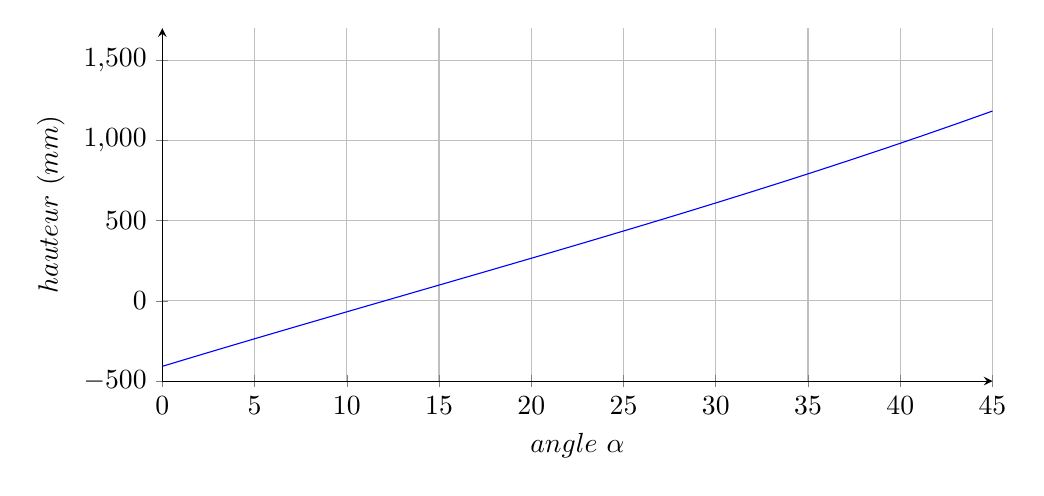
\begin{tikzpicture}
			\begin{axis}[height=0.5\linewidth, width=\linewidth,
					axis x line=bottom, axis y line=left, grid=major,
					xlabel={$angle\ \alpha$}, ylabel={$hauteur\ (mm)$},
				xmin=0, xmax=45, ymin=-500, ymax=1700]
				\addplot+[mark=none,domain=0:45] {-408.16/(cos(x)*cos(x))+2000*tan(x)};
			\end{axis}
		\end{tikzpicture}
	\end{center}
	\caption{Hauteur pour chaque angle de tir.}
	\label{crb_angle}
\end{figure}

Le problème est qu'il nous faut une fonction donnant l'angle selon la hauteur, alors que nous avons une fonction qui calcule la hauteur selon l'angle. Or la formule de cette fonction est trop complexe pour pouvoir déplacer l'angle vers la gauche de l'équation.

D'après la courbe obtenue (page~\pageref{crb_angle}), on suppose que la fonction est croissante. On peut donc procéder avec un algorithme de dichotomie afin de définir l'angle.

\newpage
\section{Démonstration de la variation de la fonction $h(\alpha)$ sur $[0;45]$.}
On découpe cette fonction en deux sous fonctions :\begin{enumerate}
	\item $h_1(\alpha) = -g*\frac{x^2}{2*\overrightarrow{v}^2*cos(\alpha)^2}$
	\item $h_2(\alpha) = x * tan(\alpha)$
\end{enumerate}
telles que $h(\alpha) = h_1(\alpha) + h_2(\alpha)$.

On ignore le $d_y$ final, car comme il est constant, il n'influencera pas le sens de variation.

Le seul intervalle considéré est $[0;45]$. Par conséquent, il m'arrivera de dire \emph{cette fonction est croissante} sans préciser l'intervalle, par abus de language.

\subsection{Analyse du sens de variation de la fonction $h_1$.}
$g$ est une constante positive, donc $-g$ est négatif.

$x^2$ est un carré, donc toujours positif.

$\overrightarrow{v}^2$ est aussi un carré donc positif, $2$ aussi est positif, donc $2*\overrightarrow{v}^2$ est positif.
Or $cos(\alpha)$ est décroissant et positif sur $[0;45]$, d'où $cos(\alpha)^2$ est décroissant.
Donc $2*\overrightarrow{v}^2*cos(\alpha)^2$ est décroissant.

Donc $\frac{1}{2*\overrightarrow{v}^2*cos(\alpha)^2}$ est croissant.

Par conséquent, comme on multiplie une valeur négative, une valeur positive et une fonction croissante, on obtient une fonction décroissante. $h_1$ est donc décroissante.

\subsection{Analyse du sens de variation de la fonction $h_2$.}
$x$ est une distance : c'est donc une valeur toujours positive.

$tan(\alpha)$ est une tangente : elle est croissante sur $[0;45]$.

En multipliant une fonction croissante par une valeur positive, on ne modifie pas le sens de variation. $h_2$ est donc croissante.

\subsection{Analyse du sens de variation de la fonction $h$.}
$h_1$ est décroissante alors que $h_2$ est croissante. On ne peut donc pas déduire la variation de leur addition. Mais lorsqu'on regarde le graphique de ces deux courbes (figure~\ref{crb_hs}, page~\pageref{crb_hs}), on constate que que $h_1$ décroit beaucoup plus lentement que $h_2$ ne croit. Par conséquent, on peut en déduire que $h$ est croissante.

On peut remarquer que ces courbes ne sont valables que pour une valeur de $x$ arbitraire. On ne peut pas être sûr que c'est vrai pour toutes ses valeurs. Pourtant lorsque qu'on observe la figure~\ref{crb_hall} (page~\pageref{crb_hall}), on remarque que le rapport entre leurs variations reste le même pour toutes les valeurs de $x$ entre $1\ m$ et $4\ m$.

On peut donc valider l'hypothèse selon laquelle $h$ est croissante (le graphique 3d de $h$ est la figure~\ref{crb_h3}).

\begin{figure}
	\begin{center}
		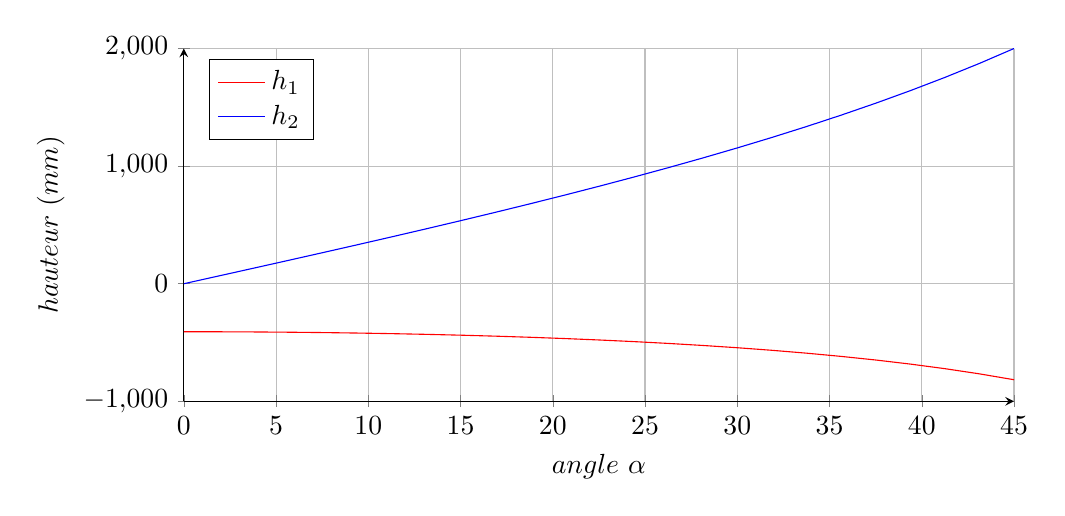
\begin{tikzpicture}
			\begin{axis}[height=0.5\linewidth, width=\linewidth,
					axis x line=bottom, axis y line=left, grid=major,
					xlabel={$angle\ \alpha$}, ylabel={$hauteur\ (mm)$},
					xmin=0, xmax=45, ymin=-1000, ymax=2000,
				legend entries={$h_1$, $h_2$}, legend style={at={(0.03,0.97)},anchor=north west}]
				\addplot+[mark=none,domain=0:45,red] {-408.16/(cos(x)*cos(x))};
				\addplot+[mark=none,domain=0:45,blue] {2000*tan(x)};
			\end{axis}
		\end{tikzpicture}
	\end{center}
	\caption{$h_1$ et $h_2$}
	\label{crb_hs}
\end{figure}

\begin{figure}
	\begin{minipage}[b]{0.45\linewidth}
		\centering
		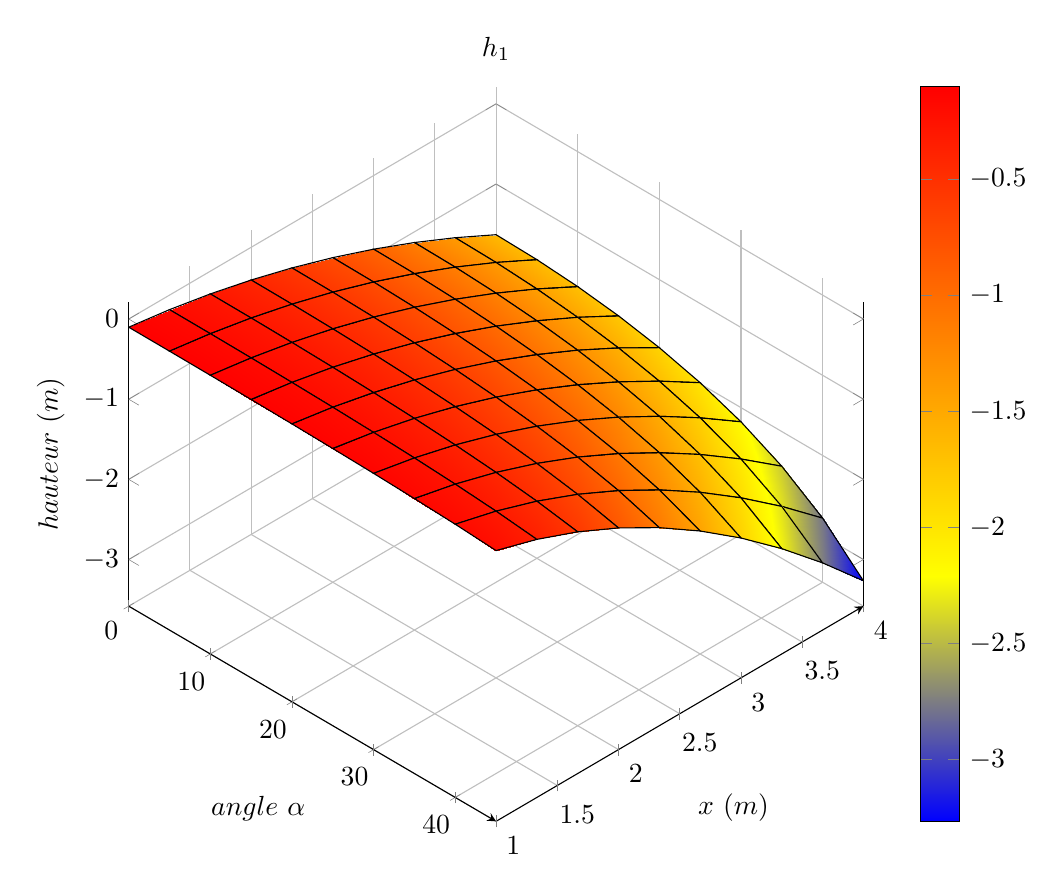
\begin{tikzpicture}
			\begin{axis}[view={45}{45},height=0.9\linewidth, width=0.9\linewidth,
					axis x line=bottom, axis y line=left, grid=major, title=$h_1$,
				xlabel={$angle\ \alpha$}, ylabel={$x\ (m)$}, zlabel={$hauteur\ (m)$},colorbar]
				\addplot3[surf,shader=faceted interp,z buffer=sort,samples=10,domain=0:45,y domain=1:4,
				faceted color=black] {-10*y*y/(98*cos(x)*cos(x))};
			\end{axis}
		\end{tikzpicture}
	\end{minipage}
	\hspace{0.5cm}
	\begin{minipage}[b]{0.45\linewidth}
		\centering
		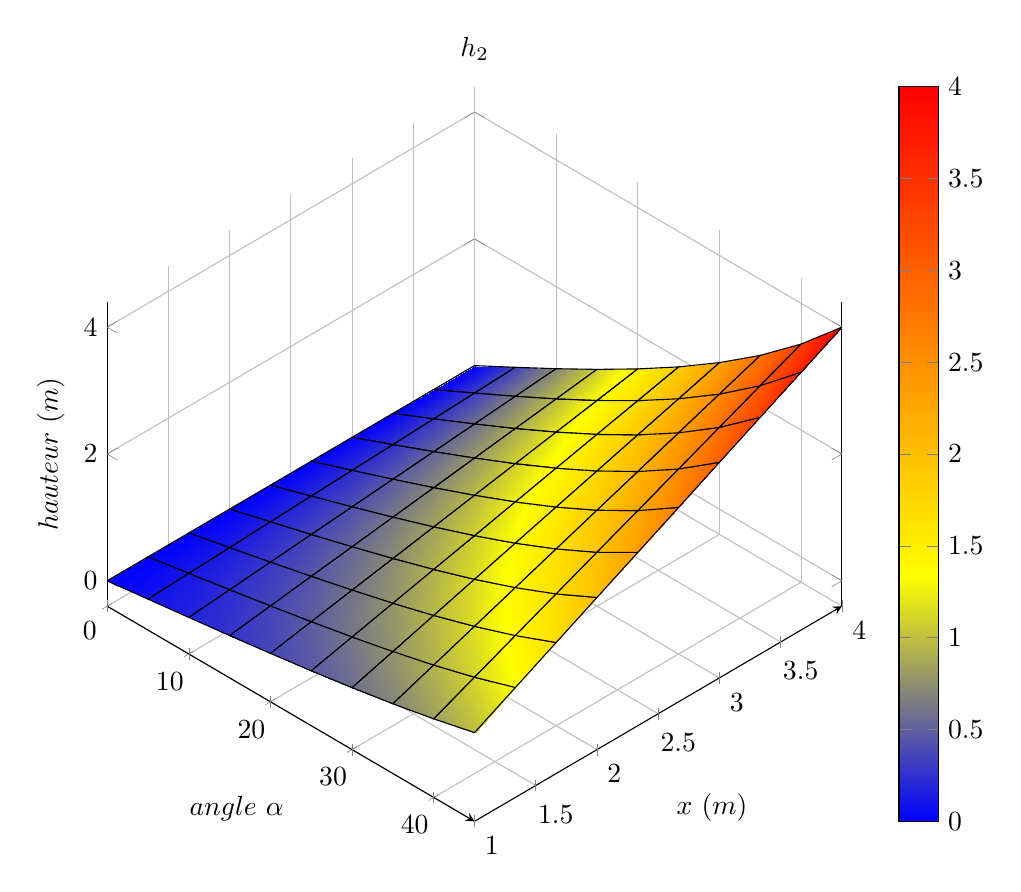
\begin{tikzpicture}
			\begin{axis}[view={45}{45},height=0.9\linewidth, width=0.9\linewidth,
					axis x line=bottom, axis y line=left, grid=major, title=$h_2$,
				xlabel={$angle\ \alpha$}, ylabel={$x\ (m)$}, zlabel={$hauteur\ (m)$},colorbar]
				\addplot3[surf,shader=faceted interp,z buffer=sort,samples=10,domain=0:45,y domain=1:4,
				faceted color=black] {y*tan(x)};
			\end{axis}
		\end{tikzpicture}
	\end{minipage}
	\caption{$h_1$ et $h_2$ en fonction de $\alpha$ et de $x$.}
	\label{crb_hall}
\end{figure}

\begin{figure}
	\begin{center}
		\centering
		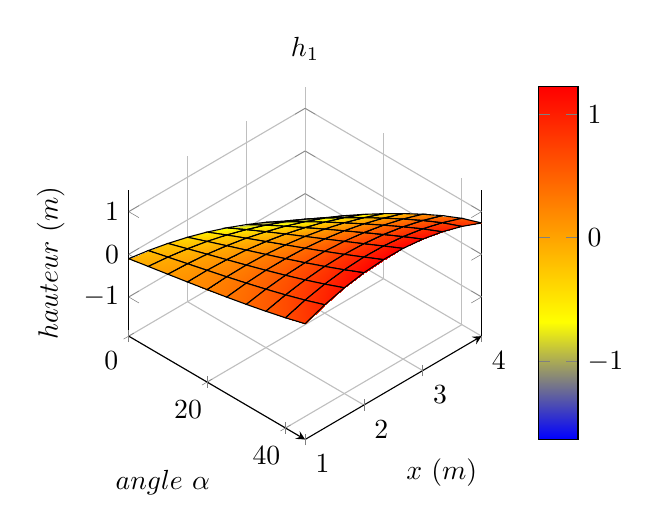
\begin{tikzpicture}
			\begin{axis}[view={45}{45},height=0.5\linewidth, width=0.5\linewidth,
					axis x line=bottom, axis y line=left, grid=major, title=$h_1$,
				xlabel={$angle\ \alpha$}, ylabel={$x\ (m)$}, zlabel={$hauteur\ (m)$},colorbar]
				\addplot3[surf,shader=faceted interp,z buffer=sort,samples=10,domain=0:45,y domain=1:4,
				faceted color=black] {-10*y*y/(98*cos(x)*cos(x))+y*tan(x)};
			\end{axis}
		\end{tikzpicture}
	\end{center}
	\caption{$h$ en fonction de $\alpha$ et de $x$.}
	\label{crb_h3}
\end{figure}
